\documentclass[11pt]{article}

%packages
\usepackage{graphicx}
\usepackage{fullpage}
\usepackage{amsmath}
\usepackage{amssymb}
\usepackage[pdfborder={0,0,0}]{hyperref}
\usepackage{pdfpages}
\usepackage[parfill]{parskip}
\usepackage{wrapfig}
\usepackage{textcomp}

\hypersetup{
    colorlinks=false,       % false: boxed links; true: colored links
    urlcolor=blue,
}

% title
%\author{Andy Barry}
%\title{}

\begin{document}

%\maketitle
\thispagestyle{empty}
\pagestyle{empty}

{\LARGE Helicopter Workshop --- Lead America Engineering and Technology Conferences}
\vspace{10pt}
\hrule
\vspace{5pt}
%Dan Barry --- Head of Faculty, Singularity University \\
Andrew Barry --- Ph.D. Candidate, Massachusetts Institute of Technology
%\\ \\
%\textbf{\large Prepared for Lead America Engineering and Technology Conferences}

\subsection*{Learning Objectives}

\begin{wrapfigure}{r}{0.5\textwidth}
    \begin{center}
    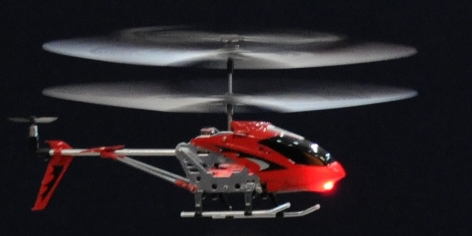
\includegraphics[width=0.48\textwidth]{figures/S107G.jpg}
    {\small S107G micro-helicopter.\footnotemark}
    \end{center}
    \vspace{-20pt}
\end{wrapfigure}
\footnotetext{\href{http://www.fiap.com.br}{FIAP, S\~ao Paulo, Brazil. 2011.}}
\textbf{1. Develop teamwork skills by building hardware and software with a group of four people.}

This workshop gives students the opportunity to collaborate on both hardware and software design by building circuitry and writing software together.  At each step, students work with each other to debug and improve their designs.  The ultimate goal of autonomous flight keeps students excited and motivated at every step.

\vspace{20pt}
\begin{wrapfigure}{r}{0.58\textwidth}
    \begin{center}
    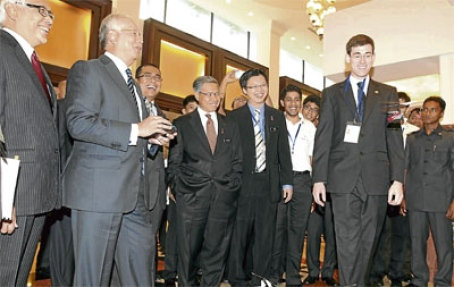
\includegraphics[width=0.58\textwidth]{figures/malaysia-prime-minister.jpg}
    {\small Malaysian Prime Minister Datuk Seri Najib Razak flies helicopter programmed by students.\footnotemark}
    \end{center}
    \vspace{-20pt}
\end{wrapfigure}
\footnotetext{\href{http://www.nst.com.my/nation/general/malaysia-gets-help-to-deal-with-food-security-issues-1.165452}{``Malaysia gets help to deal with food security issues." New Straits Times, Kuala Lumpur, Malaysia. 2012.}}

\textbf{2. Get past barriers such as, ``I can't build electronics," ``I don't know enough to write a computer program," ``I'm not smart enough to do engineering."}

Our hands-on approach shows students that they can build circuits and write software, regardless of their prior assumptions.  By \textit{doing}, students realize that they can break down large problems (fly a helicopter autonomously) into many small, solvable tasks (add an amplifier, connect the LED array, etc.).  Students leave the workshop able to reflect on their experience, realizing that they built the entire system themselves.

\newpage
\textbf{3. Learn problem-solving skills that work in a wide variety of math, science, and engineering situations.}

\begin{wrapfigure}{l}{0.5\textwidth}
    \begin{center}
    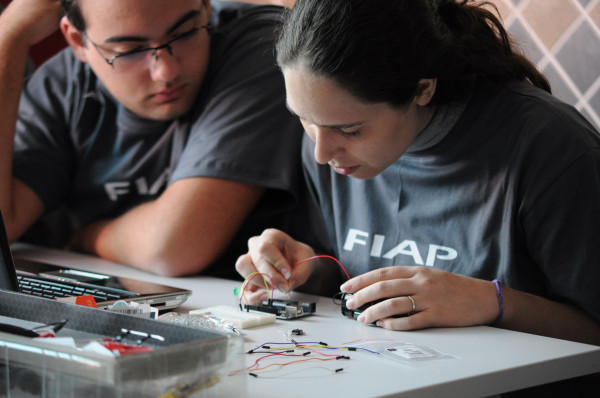
\includegraphics[width=0.48\textwidth]{figures/fiap_workshop2.jpg}
    {\small Students build a circuit.\footnotemark\vspace{10pt}}
    \end{center}
    \vspace{-20pt}
\end{wrapfigure}


Engineers apply similar skills to many problems.  Breaking down complicated issues, understanding dynamics, flying an autonomous helicopter and unwinding a unexpected result all demand similar skills.  By providing students with a skill set to understand one concrete task, they acquire the ability to solve a diverse set of problems.

%\newpage
%\vspace{20pt}
\textbf{4. Understand the full process for building and programming a useful microelectronics system.}

\footnotetext{\href{http://www.fiap.com.br}{FIAP, S\~{a}o Paulo, Brazil. 2011.}}
Microelectronics involve many layers of complexity.  When taken together, the complexity can be mind-boggling, but by breaking down each individual layer students can easily understand these systems.  We take students through every layer in their helicopter control system, allowing them to understand each component.  With knowledge of this process, the students then can grasp many other microelectronic systems.

\textbf{5. Build debugging skills for identifying, understanding, and solving common problems in these types of systems.}

Everyday, engineers work through issues on websites, airplanes, cars, and assembly lines.  Some find faults in circuitry, mechanical design, and load bearing structures.  The skills required to understand why something is not working (and how to fix it) are surprisingly similar, regardless of discipline or device.  Here, by assisting students in the debugging process, we teach them the required skills to understand and fix an issue in a complex, occasionally fast-moving, system.  Afterwards, students find these skills useful in a wide variety of applications.

\vspace{20pt}
\begin{wrapfigure}{r}{0.5\textwidth}
    \begin{center}
    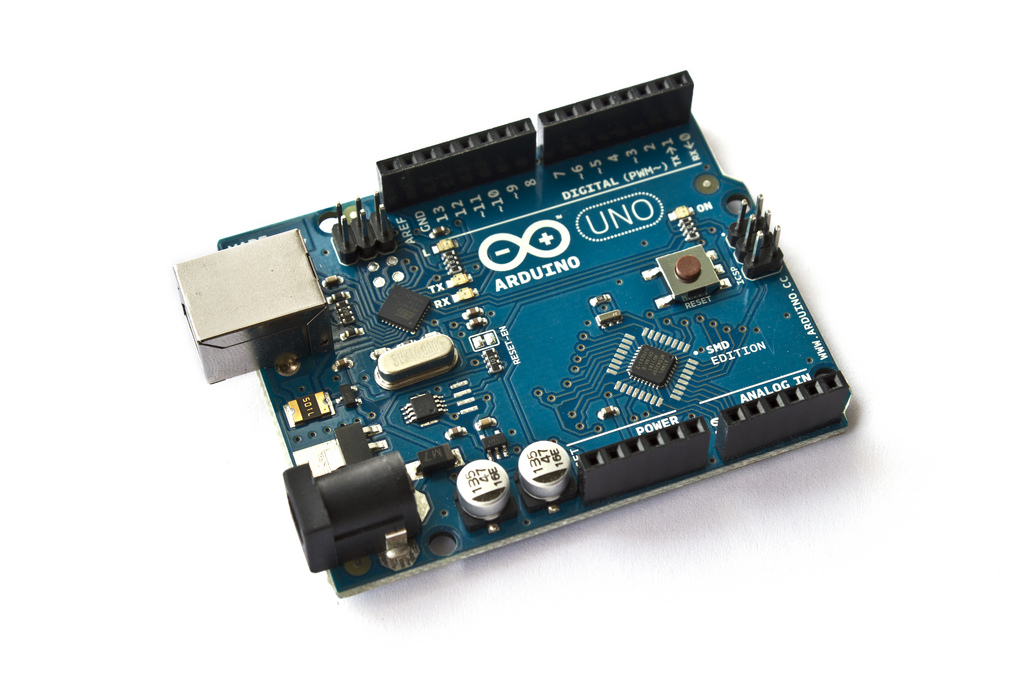
\includegraphics[width=0.48\textwidth]{figures/arduino_uno.jpg}
    {\small Microprocessor used to control the helicopters.\footnotemark}
    \end{center}
    \vspace{-30pt}
\end{wrapfigure}
\footnotetext{Image \textcopyright 2012, Justus Bl\"umer.  Used with permission.}

\textbf{6. Learn to program a microprocessor.}

At first, microprocessors are intimidating.  They can be mysterious chips, programmed in what seems like a mysterious language.  By starting with simple examples, we guide students through an introductory microprocessor programming session, building up to more complicated programs.  At the end of the workshop, students have controlled input/output ports, commanded high-level controllers, and implemented loops, conditional statements, and a variety of other constructs. 

\begin{wrapfigure}{r}{0.5\textwidth}
    \begin{center}
    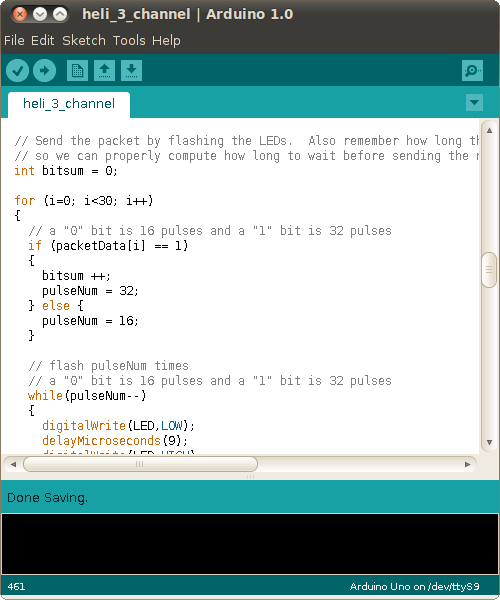
\includegraphics[width=0.48\textwidth]{figures/program.png}
    {\small Development environment for helicopter control.}
    \end{center}
    \vspace{-20pt}
\end{wrapfigure}

\textbf{7. Complete and fly an autonomous flight system.}

The workshop, in approximately four hours, guides students from start to finish through building and flying a micro-helicopter via microprocessor control.  Students are able to reflect that they can build something that, even four hours prior, seemed intimidating and impossible.

\textbf{8. Show that learning can be fun; inspire students to learn more on their own and take the skills learned in the workshop to higher levels.}

Building and programming autonomous flight systems is \textit{fun}.  Students get immediate feedback as their helicopter jumps off a table, flies into the air, and occasionally crashes to the ground.  Fast iteration promotes creative thinking, new ideas, and innovative logic.  As control code becomes more complicated, students build on their work of just minutes ago to string together complex, dynamic maneuvers.




%\section*{Workshop Summary}
%\begin{wrapfigure}{r}{0.5\textwidth}
%  \begin{center}
%    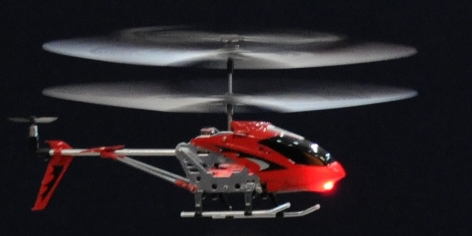
\includegraphics[width=0.48\textwidth]{figures/S107G.jpg}
%    \caption{S107G micro-helicopter. Source: \href{http://www.fiap.com.br}{FIAP, S\~ao Paulo, Brazil.}}
%  \end{center}
%\end{wrapfigure}
%Students work in small teams of approximately four members.  Each team has a computer, breadboard, microprocessor, visible LED light, infrared LED light array, battery pack, amplifier, and small helicopter.  Students start by building a simple circuit that blinks the visible LED to familiarize themselves with the different components and how to program the microprocessor.

%Once the students are accustomed to their components and environment, we guide them through the process of building a more complicated circuit that uses an amplifier to power the LED array while explaining why the microprocessor alone is unable to provide enough energy.  As they are working on their circuits, the students learn debugging techniques, such as blinking LEDs at important points in the software and utilizing a mobile phone camera to detect infrared light.

%With the circuits built and tested, the workshop transitions to discussing control systems and autonomous robotics.  Each team loads software onto their microprocessor that issues commands to their helicopters (via the IR LED array circuit they just built), but is not programmed for flight maneuvers.  The teams fly the helicopters through this interface and gain a complete understanding on the variables required for success.  We then challenge them to perform a specific autonomous maneuver with the helicopters, such as a takeoff, mid-air box, and landing.

%As teams program their systems to fly, incrementally succeeding at each step (takeoff, landing, turning, flying straight), we work with them individually to help them debug the systems and interpret the systems' outputs, especially when they are unexpected.

%For a final demonstration of the techniques, each team chooses a more complicated maneuver to fly and programs their system to perform that operation.  During this period, we discuss how feedback could make these systems better, and discuss common ways to implement feedback loops.

%The workshop closes with a summary of the vast amount of material covered and a short discussion of how these techniques are applicable to many other systems beyond flight control.

%\section*{Workshop in Detail}
%% In just four hour students learn to build circuits, program microprocessors, and write open-loop control software for micro helicopters.
%\subsection*{Step 1: How to Build Circuit}
%\begin{wrapfigure}{r}{0.4\textwidth}
%    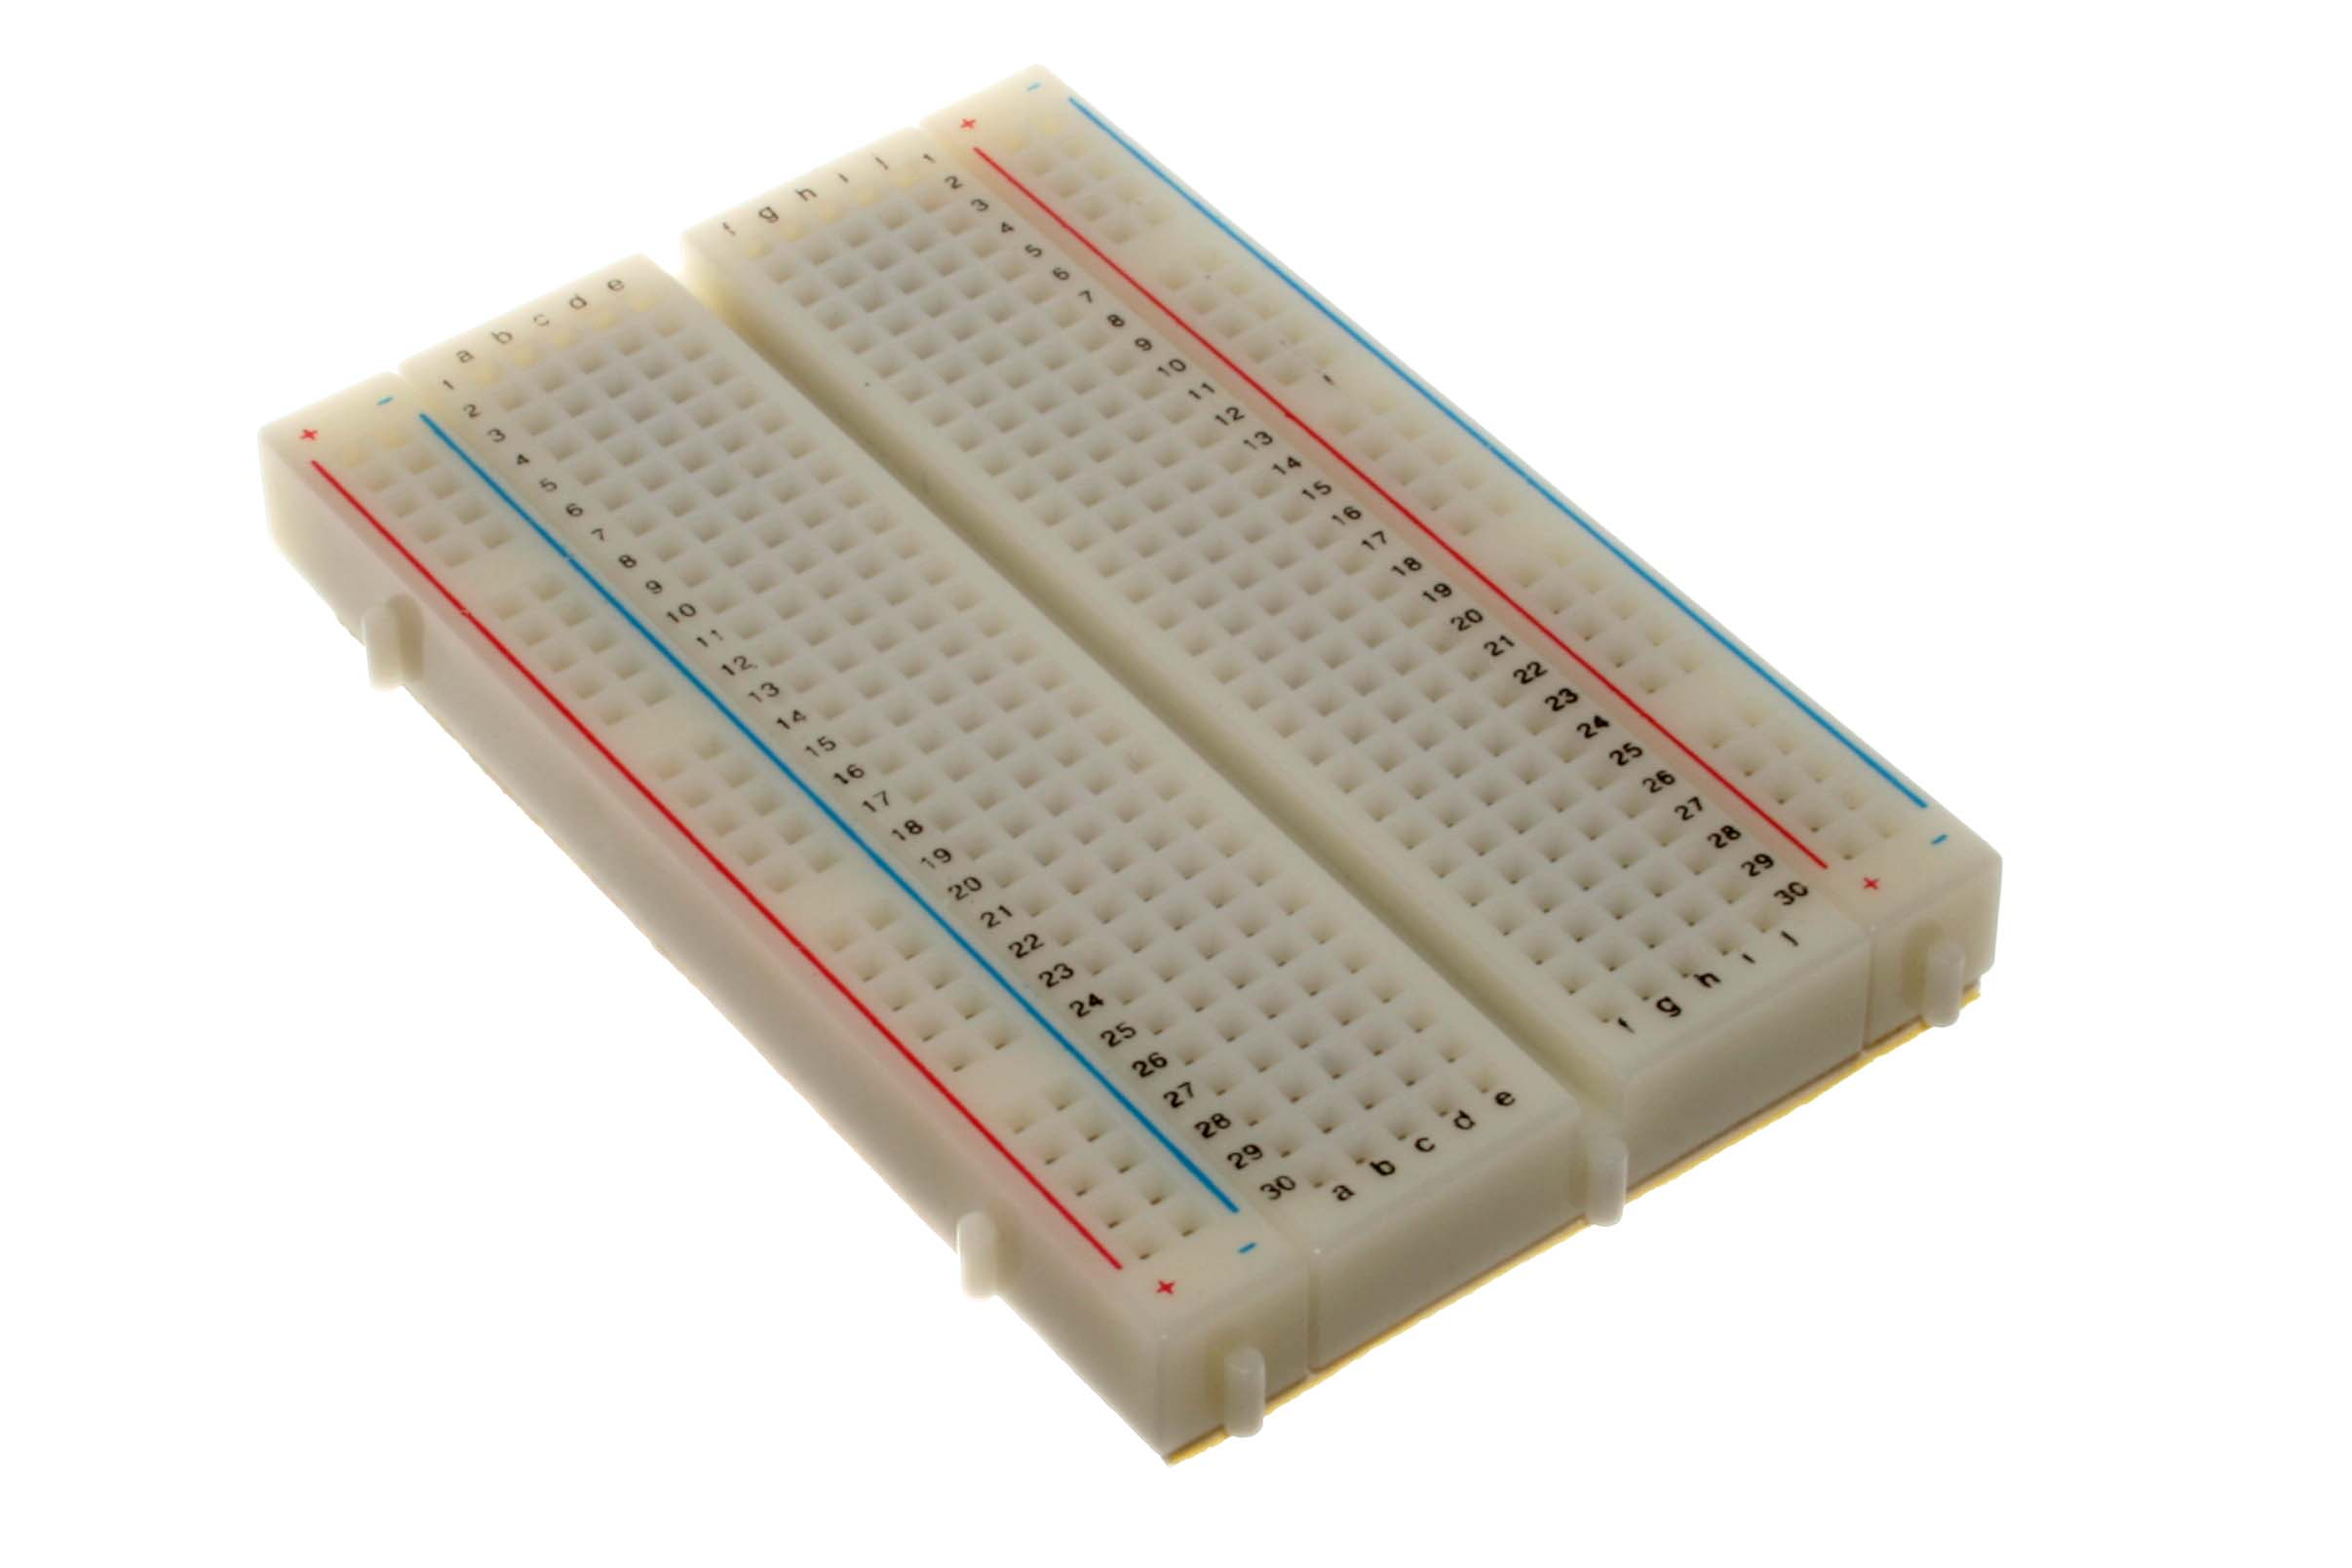
\includegraphics[width=0.38\textwidth]{figures/400_points_breadboard.jpg}
%    \caption{\label{breadboard}
%        A breadboard. Source: Oomout Ltd.
%    }
%\end{wrapfigure}
%Assuming no prior knowledge of circuit design or construction, we instruct students on circuit design and construction.  We start with how to use a breadboard (Figure \ref{breadboard}) and move on to the basic use of a mircoprocessor.  Each group builds a simple circuit and programs their microprocessor to blink a light.





%\begin{thebibliography}{1}

%\bibitem{bookName}
% Book

%\end{thebibliography}

%\begin{figure}
%\includegraphics[width=\textwidth]{}
%\caption{
%    Caption
%    \label{fig}
%}
%\end{figure}

%\includepdf[pages=-]{}

%\begin{table}
%\begin{tabular}{|r|r|}
%\hline
%Col Header 1&Col Header 2\\
%\hline
%4&18\\
%5&24\\
%6&22\\
%7&35\\
%\hline
%\end{tabular}
%\caption{
%    Table
%    \label{table}
%}
%\end{table}

\end{document}

